% NOTES:
%%    do we want to explore for larger S?  Does false positive rate change?

% TODO:
%   reference tables!!

\documentclass{pnastwo}
\usepackage[pdftex]{graphicx}
\graphicspath{{figures/}}

\begin{document}

\title{Scaling metagenome sequence assembly with probabilistic de Bruijn
graphs}

\author{
Jason Pell
\affil{1}{Michigan State University, East Lansing, MI, United States}
\and
Arend Hintze
\affil{1}{}
\and
Rosangela Canino-Koning
\affil{1}{}
\and
Adina Howe
\affil{1}{}
\and
James M. Tiedje
\affil{1}{}
\and
C. Titus Brown
\affil{1}{}
}

\maketitle

%{\center
%Classification:\\
%Physical Sciences, Computer Sciences;\\
%Biological Sciences, Biophysics and Computational Biology\\
%}

\begin{article}

\begin{abstract}

The memory requirements for de novo assembly of short-read shotgun
sequencing data from complex microbial populations are an increasingly
large practical barrier to environmental studies.  Here we introduce a
simple probabilistic graph representation for de Bruijn assembly
graphs based on Bloom filters.  This data structure can store assembly
graphs with 4 bits per k-mer, independent of the specific k -- a
dramatic improvement over current approaches.  We show that despite
the false positive nodes and edges in the graph resulting from the
representation, it can be used to scale partitioning, a ``divide and
conquer'' approach to metagenome assembly.

\end{abstract}

\keywords{metagenomics | de novo assembly | de Bruijn graphs | k-mers}

\section{Introduction}

De novo assembly of shotgun sequencing reads into longer contiguous
sequences plays an important role in virtually all genomic research.
However, current computational methods for sequence assembly do not
scale well to the volume of sequencing data now readily available from
next-generation sequencing machines.  In particular, the deep
sequencing required to sample complex microbial environments easily
results in data sets that surpass the working memory of available
computers.

Shotgun sequencing produces hundreds of millions or billions of short
sequences that are randomly read from the sample, and assembly of
these short sequences into longer, non-redundant sequences is
critically important for gene content analysis.  The process of
sequence assembly relies upon overlap analysis between many short
sequences, and efficient overlap analysis in turn requires a
substantial amount of working memory in order to store these overlaps.

Assembly of short reads is particularly important for the sequencing
and analysis of complex microbial ecosystems, which can contain
thousands and even millions of individual microbial species.  These
ecosystems mediate important biogeochemical processes but are still
poorly understood at a molecular level, in large part because they
consist of many microbes that cannot be cultured or studied
individually in the lab.  Ensemble sequencing (``metagenomics'') of
these complex environments is one of the few ways to render them
accessible, and has resulted in substantial early progress in
understanding the composition and function of the human gut, cow
rumen, and permafrost soil.  However, as sequencing capacity grows,
the assembly of sequences from these complex samples has become
increasingly computationally challenging.  Current methods for assembly rely on
inexact data reduction in which reads from low-abundance organisms are
discarded, biasing our analysis towards high-abundance organisms.

% @@ newbler fix
% @@ cite jansson paper

The predominant assembly formalism applied to short-read sequencing
data sets is a de Bruijn graph \cite{pubmed20211242,pubmed22068540}.
In a de Bruijn graph approach, sequencing reads are decomposed into
fixed-length words, or k-mers, and used to build a connectivity graph.
This graph is then traversed to determine contiguous sequences
\cite{pubmed22068540}.  Because de Bruijn graphs store only k-mers,
memory usage scales with the number of unique k-mers in the data set
rather than the number of reads.  Thus human genomes can be assembled
in as little as 512 GB of system memory \cite{pmid21187386}.  For more
complex samples such as soil metagenomes, which may possess millions
or more species, terabytes of memory would be required to store the graph
\cite{pubmed21304727}.

In this work, we describe a simple probabilistic representation for
storing de Bruijn graphs in memory, based on Bloom filters
\cite{bloom}.  Bloom filters are constant-memory probabilistic data
structures for storing sets; essentially hash tables without collision
detection, set membership queries on Bloom filters can yield false
positives -- k-mers marked as present that do not actually exist --
but not false negatives.  We show that this probabilistic graph
representation can be used to efficiently store and traverse DNA de
Bruijn graphs with an approximately 20-fold decrease in memory usage
over the Velvet and ABySS assemblers. We relate changes in local and
global graph connectivity to the false positive rate of the underlying
Bloom filters, and show that the graph's global structure is accurate
until an abrupt transition in false connectivity near a false positive
rate of 0.183, corresponding to a lower memory limit of approximately
4 bits per graph node.

We also show that this graph representation can be used to accurately
assemble a soil metagenome in substantially reduced memory, through
the use of partitioning.  Partitioning is an approach in which the de
Bruijn graph is divided up into components, and in the past it has
been used to improve the quality of transcriptome and metagenome assemblies,
but not to scale the assembly process itself.
\cite{trinity, metavelvet,pubmed21685107}.  By applying the
probabilistic de Bruijn graph representation to the problem of
partitioning, we can achieve a dramatic decrease in the memory
required for assembly.

% @@ exact/inexact data influence

\section{Results}

\subsection{Bloom filters can store de Bruijn graphs}

Given a set of short DNA sequences, or reads, we first break down each
read into a set of overlapping k-mers.  We then store each k-mer
in a Bloom filter.  Each k-mer serves as a vertex in a graph, with an edge
between two vertices $N_1$ and $N_2$ if and only if $N_1$ and $N_2$
share a (k-1)-mer that is a prefix of $N_1$ and a postfix of $N_2$,
or vice versa (see Figure \ref{fig:bloomgraph}).  This edge is not stored explicitly.

Thus each k-mer has up to 8 neighbors, which can be determined by
simply building all possible 1-base extensions and testing for their
presence in the Bloom filter.  In doing so, we implicitly treat
the graph as a simple graph as opposed to a multigraph or digraph,
which means that there can be no self-loops or parallel edges between
vertices/k-mers. This graph representation is constant in its memory
usage, so only ancillary information such as list of vertices visited
or waypoints in the graph consumes additional memory.
By relying on Bloom filters, the data structure is constant
memory: no extra memory is used as additional data is added. However,
as memory is decreased or data is increased, false positive vertices
and edges are gained, so compressing the graph results in a more
tightly interconnected graph.

This graph structure is effectively {\em compressible} because one can
choose a larger or smaller size for the underlying Bloom filters; a
larger size admits fewer false positives, while a smaller size admits
more. In exchange, we can store k-mer nodes more or less efficiently: for
example, for a false positive rate of 15\%, at which 1 in 6 random k-mers
tested would be falsely considered present, each k-mer can be stored
in under 4 bits of memory (see Table \ref{table:bitskmer}).

In contrast to an exact graph storage, there is a chance that a k-mer will
be adjacent to a false positive: that is, a k-mer may connect to another k-mer that does not
actually exist in the original dataset but nonetheless registers as present,
due to the probabilistic nature of the Bloom filter.  If the false positive rate is too high, the graph structure will
be dominated by false connectivity -- but what rate is ``too high''?  We study this in detail below.

\subsection{False positives cause local elaboration of graph structure}

Erroneous neighbors created by false positives can alter the graph
structure.  To better understand this effect, we generated a random
1,031bp circular sequence and visualized the effect of different false
positive rates.  After storing this single sequence in compressible
graphs using $k=31$ with four different false positive rates
($p_f$=0.01, 0.05, 0.10, and 0.15), we explored the graph using
breadth-first search beginning at the first 31-mer.  The graphs in
Figure \ref{fig:circles} demonstrate how the local graph structure elaborates with the
false positive rate while the overall circular graph structure
remains, with no erroneous shortcuts between k-mers that are present
in the original sequence.  It is visually apparent that even a high false positive rate of 15\% does not systematically and erroneously connect distant k-mers.

In addition, it is simple to see that a linear increase in the false 
positive rate results in a linear increase in the number of expected 
neighbors for a particular k-mer. For most isolated k-mers (i.e. no adjacent 
``real'' k-mers), the calculation is 
E(erroneous neighbors)$ = 8 \times p_f$. Thus, the local graph 
structure breaks down in a linear fashion.  Does the global graph structure
degrade in a similar fashion?

\subsection{False long-range connectivity is a nonlinear function of the false positive rate}

To explore the point at which our data structure systematically
engenders false long-range connections, we inserted random 31-mers
into Bloom filters with increasing false positive rates.  We then
estimated the average cluster size for each false positive rate
($n=10000$) and used percentile bootstrap to obtain estimates within a
95\% confidence interval. Figure \ref{fig:clustersize} demonstrates that the average cluster size
rapidly increases as a specific threshold is approached, which appears
to be at a false positive rate near 0.18 for k=31. Beyond 0.18, the components
begin to join together as a single giant cluster, and small components
are more rare.

As the false positive rate increases, we observe a sudden transition
from many small components to fewer, larger components created by erroneous connections between the ``true'' components (Figure \ref{fig:clustersize}).  In contrast to the linear increase in the
local neighborhood structure as the false positive rate increases
linearly, the change in global graph structure is abrupt as previously
disconnected clusters join together.  This rapid change resembles a
phase transition, which for graphs can be discussed in terms of
percolation theory. We can map our problem to site percolation by
considering a probability $p$ that a particular k-mer is the ``on''
state. (This is in contrast to bond percolation where $p$ represents
the probability of a particular edge being in the ``on'' state.) As
long as the false positive rate is below the percolation threshold
$p_\theta$ (i.e. in the subcritical phase), we would predict that the graph
is not highly connected by false positives.

% @CTB MENTION ITERATIVE PARTITIONING

Percolation thresholds for finite graphs can be estimated by finding
where the cluster size distribution transitions from linear to
quadratic in form \cite{stauffer1979scaling}.  Using the calculation
method described in \emph{Methods}, we found the site percolation
threshold for DNA de Bruijn graphs to be $p_\theta = 0.183 \pm 0.001$.
Although we only tested within a limited range of k from 20 to 32, the
percolation threshold appears to be independent of different $k$.
Thus, as long as the false positive rate is below $0.183$, we
predict that truly disconnected components in the graph are unlikely
to connect to one another erroneously, that is, due solely to errors
introduced by the probabilistic representation.
%% @@do we need to demonstrate k independence anywhere?

\subsection{Large-scale graph structure is retained to the percolation threshold}

The results from cluster size analysis and the percolation threshold
estimation suggest that global connectivity of the graph is unlikely
to change below the percolation threshold. To verify this, we employed
the diameter metric in graph theory.  The diameter of a component in a
graph is a measure of the length of the ``longest shortest'' path
between any two vertices\cite{bondy2008graph}.  In our case, we only
considered paths between two real k-mers in the dataset.  We randomly generated 58bp long
circular chromosomes to construct components containing 50 8-mers and
calculated the diameter at different false positive rates. At each
false positive rate, we ran the simulation 500 times and estimated the
mean within a 95\% confidence interval using percentile bootstrap. As Figure \ref{fig:diam} shows, erroneous
connections between pairs of real k-mers are rare below the
percolation threshold. For false positive rates at or above the
percolation threshold, spurious connections between real k-mers are
created, which lowers the diameter.  Thus, the larger scale graph
structure is retained through $p > 0.183$, as suggested by the cluster
size analysis and percolation results.

\subsection{Sequencing errors eclipse false positives}

One important consideration for the utility of the de Bruijn graph
representation is to compare it with graphs built from real data from
massively parallel sequencers such as Illumina, which contain base
calling errors.  In de Bruijn graph-based assemblers, these sequencing
errors add to the graph complexity and make it more difficult to find
high-quality paths for generating long, accurate contigs. Since our
approach also generates false positives, we wanted to compare the
error rate from the Bloom filter graph with experimental errors
generated by sequencing (Table \ref{table:ecoli}). We used the \emph{E. coli} K-12
MG1665 genome to compare various graph invariants between an Illumina
dataset generated from the same strain (see \emph{Methods}), an exact
representation of the genome, and inexact representations with
different false positive rates.

For these comparisons, we used a $k$ value of 17, which allows us to
use Bloom filters with no false positives.
We found a
total of 50,605 17-mers in the exact representation that were not part
of a simple line, i.e. had more than two neighbors (degree $>$ 2). As
the false positive rate increased, the number of these 17-mers
increased in the expected linear fashion.
% in addition to the number of
%false positive 17-mers found in each component.
Furthermore, the
number of real 17-mers, those that are not false positives,
comprise the majority of the graph.

In contrast, when we examined an exact representation of an Illumina
dataset, only 9.9\% of the k-mers in the graph truly exist in the
reference genome.  As above, we only counted false positive k-mers
that are transitively connected to least one real k-mer. The number of
17-mers with more than 2 neighbors is higher than for the exact
representation of the genome, which demonstrates that sequencing
errors add to the complexity of the graph. Overall, the
errors demonstrated by sequencers dwarf the errors caused by the
inexact graph representation below a reasonable false positive rate.

When we assemble this data set with the Velvet and ABySS assemblers at
k=31, Velvet requires 3.7gb to assemble the data set,
while ABySS requires 1.6gb; this memory usage is dominated by the
graph storage \cite{zerbinothesis}. Thus the Bloom filter approach stores graphs 40 or
more times more efficiently than either program, even with a low false
positive rate of 1\%.  While this is not a perfect comparison -- assemblers do more than simply store the graph! -- it does directly suggest that 

\subsection{Sequences can be accurately partitioned by graph connectivity}


Can we use this lightweight graph representation to find and separate
components in de Bruijn graphs?  The primary concern is that false positive
nodes or edges would connect components, but the diameter results suggest that
components are unlikely to connect below the percolation
threshold. To verify this, we analyzed a simulated dataset of 1,000
randomly generated sequences of length 10,000 bp.  Using $k=31$,
we partitioned the data across many different false positive rates,
using the procedure described in \emph{Methods}. As predicted, the
resulting number of partitions did not vary across the false positive
rates while $f_p \le 0.15$ (Figure \ref{fig:partfp}).

We then applied partitioning to a considerably larger bulk soil
metagenome (``MSB2'') containing 35 million 75 bp long reads generated
from an Illumina GAII sequencer.  We calculated the number of unique
31-mers present in the data set to be 1.35 billion. Then, for each of
several false positive rates (see Table \ref{table:parts}) we loaded
the reads into a graph, eliminated components containing fewer than
500 unique k-mers, and partitioned the reads into separate files based
on graph connectivity.

Once we obtained the partition sets, we individually assembled each
set of partitions, as well as the entire (unpartitioned) data set,
retaining contigs longer than 500 bp.  The resulting assemblies were
all identical, containing 1,444 contigs with a total assembled
sequence of 1.07 mb.  The unpartitioned data set required 33 GB to
assemble with ABySS, while the partitioned data sets all required
under 1.5 GB to partition and assemble -- an improvement of over
20-fold for an identical result.

% @CTB repartitioning

\section{Discussion}

% @@ reorder so concluding thoughts come up top? naah.

\subsection{Bloom filters can be used to efficiently store de Bruijn graphs}

The use of Bloom filters to store an implicit de Bruijn graph is
straightforward and memory efficient.  The expected false positive
rate can be tuned based on hash table occupancy, yielding a wide range
of possible storage efficiencies.

Even for low false positive rates such as 5\%, this is still an
efficient graph representation, with a greater than 20-fold improvement
in memory usage over two existing assemblers, Velvet and ABySS.  The false
positive rates have a small effect on branching graph structure
compared to sequencing errors, suggesting that this is an effective
practical representation for de Bruijn graphs.  In addition, the false positives
engendered by the Bloom filters are uncorrelated with the original
sequence, unlike sequencing errors which usually have a low edit
distance to the real sequence.  This feature may further reduce the effect of
false positives on de Bruijn graph analysis, depending on the specific
application.

\subsection{Preservation of long-range structure permits graph partitioning}

Using a probabilistic graph representation with false positive nodes
and edges raises the specter of systematic graph artifacts resulting
from the false positives.  For partitioning, the primary concern is that false
positives will incorrectly connect components, rendering partitioning
ineffective.  Our results from percolation analysis, diameter
calculations, and partitioning of simulated and real data demonstrate that
below the calculated percolation threshold this is not a significant
problem.  As long as the expected rate of false edges is sufficiently
low, long false paths are not spontaneously created and hence the
large scale graph properties do not change.

Our partitioning results on a real metagenome, the MSB2 data set,
demonstrate the utility of partitioning for reducing memory usage.
For this specific data set, we obtained {\em identical} results with a
20-40x decrease in memory (Table \ref{table:parts}).  This is consonant with our results from
storing the E. coli genome, in which we achieved a 20-fold decrease
in memory usage over the exact representation at a false positive rate
of 1\%.  While increased coverage and variation in data set complexity
will affect the actual memory usage, these results demonstrate that
significant scaling in the memory required for assembly can be achieved
in at least one case.

The memory requirements for the partitioning process for the MSB2 data
set are dominated by the memory required to store and explore the
graph; the higher memory usage for partitioning at a false positive rate
of 15\% is due to the increase in component size from local false
positives.  In particular, the memory requirements for downstream assembly
of partitions is driven by the size of the largest partition, which
here is very small (345,000 reads; Table \ref{table:parts}).  The
dominant partition size is remarkably refractory to the graph's false
positive rate, increasing by far less than 1\% for a 15-fold increase
in false positives; this shows that our theoretical and
simulated results for cluster size and diameter apply to the MSB2 data set
as well.

% @CTB fill in number

There are several biological problems that are particularly well
suited to a partitioning approach.  Like metagenomes, transcriptomes
consist of populations of many {\em disconnected} sequences.  This has
already been exploited for assembly improvement: Trinity relies on a
partitioning approach in the second phase of transcriptome assembly;
and both Meta-IDBA and MetaVelvet rely on locality of coverage and and
discovery of components for metagenome assembly
\cite{trinity,pubmed21685107,metavelvet}.  These algorithms, however,
rely on exact graph representations that are more memory intensive
than the one presented here.  The utility of the probabilistic graph
representation for partitioning rests on its significantly lower
memory usage.

Combined with the scaling
properties of the graph representation, partitioning with this probabilistic
de Bruijn graph representation offers a way to
efficiently apply a ``divide and conquer'' strategy to certain
assembly problems.  While this work focuses on theoretical properties
of the graph representation, the next step will be to evaluate the approach
on many real data sets.

\subsection{Concluding thoughts}

% @@ mention utility for trinity, etc.
% @@ read, cite references from pop

Developing efficient and accurate approaches to de novo assembly
continues to be one of the ``grand challenges'' of bioinformatics,
with significant implications for investigation of life on Earth, much
of which has not been sampled (cite).  While our appreciation is
growing for the role that microbes play in biogeochemical processes,
we are increasingly limited by our ability to analyze the data.  For
example, the Earth Microbiome Project is generating petabytes of
sequencing data from complex microbial communities, many of which
contain entirely novel ensembles of microbes; scaling de novo assembly
is a critical part of this investigation (cite).  Furthermore, scaling
de novo assembly should result in improved assemblies, as it will
allow more compute-intensive algorithms to be applied; this is
especially true for divide-and-conquer approaches, which scale
dramatically.

The probabilistic de Bruijn graph representation presented here has a
number of convenient features for storing and analyzing large assembly
graphs.  First, it is efficient and compressible: for a given data
set, a wide range of false positive rates can be chosen without
impacting the global structure of the graph, allowing graph storage in
as little as 4 bits per k-mer.  Because a higher false positive rate
yields a more elaborate local structure, memory can be traded for
traversal time in e.g. partitioning.  Second, it is a constant memory
data structure, with predictable degradation of both local and global
structure as more data is inserted.  For data sets where the number of
unique k-mers is not known in advance, the occupancy of the data
structure can be monitored as data is inserted and directly converted
to an expected false positive rate.  Third, the memory usage is
independent of the k-mer size chosen, making this representation
convenient for exploring properties at many different parameters.  It
also allows the storage and traversal of de Bruijn graphs at multiple
k-mer sizes within a single structure, although we have not yet
explored these properties.

Our initial motivation for developing this use of Bloom filters was to
explore partitioning as an approach to scaling metagenome assembly,
but there are many additional uses beyond metagenomics.  Partitioning
has been applied to mRNAseq assembly as well, so this graph representation also be
useful for scaling transcriptome assembly \cite{trinity}.  In general
a more memory efficient de Bruijn graph representation could open up
many opportunities.  While de Bruijn graph approaches are currently
being used primarily for the purposes of assembly, they are a broadly
useful formalism for sequence analysis. In particular, they have been
extended to efficient multiple-sequence alignment\cite{zhang2003dna},
repeat discovery\cite{price2005novo}, and detection of local and
structural sequence variation \cite{zerbinothesis}.  We are also
exploring the use of de Bruijn graphs for graph-based homology search
and artifact detection in large sequencing data sets.  The ability to
scale graph storage by a factor of 10 or more may also result in
additional uses for de Bruijn graphs.

%While de Bruijn graphs have traditionally been viewed as
%heavy weight computational solutions due to the extremely large memory
%requirements, our initial investigations into the PDBG described here
%demonstrate a $\approx$ 20-fold decrease in memory requirements over
%Velvet.  This may translate into similar memory savings in these other
%applications.  One significant caveat to this reduced memory usage is
%that as only the graph structure itself is stored in the Bloom
%filters, additional information such as node weights and traversal
%waypoints will take up additional memory.  Such questions remain to be
%explored in future work.

\begin{materials}

\section{Genome and Sequence Data}
We used the \emph{E. coli} K-12 MG1655 genome (GenBank: U00096.2) and two MG1655 Illumina 
datasets (Short Read Archive accessions SRX000429 and SRX000430) for E. coli
analyses.

\section{Data Structure Implementation}
We implemented a variation on the Bloom filter data structure to store
k-mers in memory. In a classic Bloom filter, multiple hash functions
map bits into a single hash table to add an object or test for the presence
of an object in the set. In our variant, we use multiple
prime-number-sized hash tables, each with a different hash
function corresponding to the modulus of the DNA bitstring
representation with the hash table size; this is a computationally convenient way to construct hash functions for DNA strings.  The underlying properties of
the Bloom filter are identical.  To add a k-mer to the
filter, the corresponding bit is set to 1 in each hash table.  To find
the presence of a k-mer, each table is queried for the presence of
that k-mer; for a k-mer to be considered present in the dataset, the
k-mer must be found in all of the hash tables.  If a k-mer is not
present in any one hash table, then it is certainly not in the
dataset. This explains the one-sided error: false positives are
possible but false negatives are not. The expected false positive rate
is simply the product of the occupancies of the hash tables.  As with
other hash-style data structures, Bloom filters have a fast lookup
time, $O(h)$ for $h$ hash tables.  Similar to other hash-style data
structures for storing k-mers, memory usage is independent of the
value of $k$.

\section{Calculating Data Structure Properties}
The properties of our Bloom filter variant are the
same as a classical Bloom filter \cite{bloomsurvey}.
To calculate the expected false positive 
rate, we
take the product of the occupancy of each hash table:
\begin{displaymath}
P_f = \prod_{h \in H} occ(h)
\end{displaymath}
where $h$ is a hash table in the set of hash tables $H$ and $occ$ denotes
the occupancy (proportion of bits set) for a hash table.
We find the optimal number of hash tables
to use by calculating
\begin{displaymath}
\vert H \vert_{opt} = \ln 2 \frac{m}{k}
\end{displaymath}
where $m$ is the amount of memory in bits to allocate and $k$
is the number of unique k-mers to be inserted. Finally,
the number of bits per
k-mer used in the data structure for the optimal number of hash 
tables is

\begin{displaymath}
\frac{m}{n} = \frac{1}{\ln(2)} \log{\frac{1}{P_f}}.
\end{displaymath}

\section{Estimating False Positive Rate For Erroneous Connectivity}
We ran a simulation to find when components in the graph 
begin to erroneously connect to one another.
To calculate the false positive rate $p$ at which this aberrant 
connectivity occurs, 
we added random k-mers, sampled from a uniform GC distribution, to the data structure 
and then calculated the occupancy and size of 
the largest 
component. From this we sampled the relative size of 
the largest component and the overall cluster size distribution for each
given occupancy rate.
At the occupancy where a ``giant cluster'' appears, this cluster size distribution 
should be scale-free \cite{stauffer1979scaling}. 

We then found at what value of $p$ the resulting 
cluster size distribution in logarithmic 
scale can be better fitted in a linear or quadratic fashion using 
the F-statistic
\newline
\newline
\begin{displaymath}
F=\frac{RSS_1-RSS_2}{p_2-p_1} \times \frac{n - p_2}{RSS_2}
\end{displaymath}

where $RSS_i$ is the residual sum of squares for model $i$, $p_i$ is 
the number of parameters for model $i$, and $n$ is the number of data 
points. To handle the finite size sampling error, the data was binned using the 
threshold binning method \cite{adami2002critical}. The critical value for 
when aberrant connectivity occurred was found by determining the local maxima 
of the F-values \cite{wald43}.

\section{Graph Partitioning Using A Bloom Filter}

We used the Bloom filter data structure containing the k-mers from a
dataset to discover components of the graph, i.e. to partition the
graph.  Here a component is a set of k-mers whose originating reads
overlap transitively by at least $k$ base pairs.  Reads belonging only
to small components can be discovered and eliminated in constant
memory using a simple traversal algorithm that truncates after
discovering more than a given number of novel k-mers.  For discovering
large components we tag the graph at a minimum density by using the
underlying reads as a guide.  We then exhaustively explore the graph
around these tags in order to connect tagged k-mers based on graph
connectivity.  The underlying reads in each component can then be
separated based on their partition.

\section{Assembler software}

We used ABySS v1.3.1 and Velvet v1.1.07 to perform assemblies (cite).
The ABySS command was: {\tt mpirun -np 8 ABYSS-P -k31 -o contigs.fa reads.fa}.
The Velvet commands were: {\tt velveth test 31 -fasta -short reads.fa \&\& velvetg test}.
We did not use Velvet for the partitioning analysis because Velvet's
error correction algorithm is stochastic and results in dissimilar
assemblies for different read order.

\section{Software and Software Availability}

We have implemented this compressible graph representation and the associated
partitioning algorithm in a
software package named khmer.  It is written in C++ and Python 2.6 and
is available under the BSD open source license at
https://github.com/ctb/khmer.  The graphviz software package was used
for graph visualizations. The scripts to generate the figures of this
paper are available in the khmer repository.

\end{materials}

\begin{acknowledgments}

We thank Chris Adami, Qingpeng Zhang, and Tracy Teal for
thoughtful comments, and Jim Cole and Jordan Fish for discussion of future
applications.  This project was supported by AFRI Competitive Grant
no. 2010-65205-20361 from the USDA NIFA, and NSF IOS-0923812.  The
MSB2 soil metagenome was sequenced by the DOE's Joint Genome
Institute through the Great Lakes Bioenergy Research Center.

\end{acknowledgments}

% @@CTB mention k_0 > k_1 etc.

\bibliographystyle{abbrv}

\begin{thebibliography}{10}

\bibitem{adami2002critical}
C.~Adami and J.~Chu.
\newblock {C}ritical and near-critical branching processes.
\newblock {\em Physical Review E}, 66(1):011907, 2002.

\bibitem{bloom}
B.~Bloom.
\newblock {{S}pace/time tradeoffs in hash coding with allowable errors}.
\newblock {\em CACM}, 13(7):422--426, 1970.

\bibitem{bondy2008graph}
J.~Bondy and U.~Murty.
\newblock {G}raph {T}heory.
\newblock {\em Graduate Texts in Mathematics}, 2008.

\bibitem{bloomsurvey}
A.~Broder and M.~Mitzenmacher.
\newblock {N}etwork applications of bloom filters: {A} survey.
\newblock {\em Internet Mathematics}, 1(4):485--509, 2004.

\bibitem{pubmed22068540}
P.~Compeau, P.~Pevzner, and G.~Tesler.
\newblock How to apply de bruijn graphs to genome assembly.
\newblock {\em Nat Biotechnol}, 29(11):987--91, 2011.

\bibitem{zerbinothesis}
Z.~DR.
\newblock Genome assembly and comparison using de bruijn graphs (phd thesis).
\newblock 2009.

\bibitem{pubmed21304727}
J.~Gilbert, F.~Meyer, D.~Antonopoulos, P.~Balaji, C.~Brown, C.~Brown, N.~Desai,
  J.~Eisen, D.~Evers, D.~Field, W.~Feng, D.~Huson, J.~Jansson, R.~Knight,
  J.~Knight, E.~Kolker, K.~Konstantindis, J.~Kostka, N.~Kyrpides,
  R.~Mackelprang, A.~McHardy, C.~Quince, J.~Raes, A.~Sczyrba, A.~Shade, and
  R.~Stevens.
\newblock Meeting report: the terabase metagenomics workshop and the vision of
  an earth microbiome project.
\newblock {\em Stand Genomic Sci}, 3(3):243--8, 2010.

\bibitem{pmid21187386}
S.~Gnerre, I.~Maccallum, D.~Przybylski, F.~J. Ribeiro, J.~N. Burton, B.~J.
  Walker, T.~Sharpe, G.~Hall, T.~P. Shea, S.~Sykes, A.~M. Berlin, D.~Aird,
  M.~Costello, R.~Daza, L.~Williams, R.~Nicol, A.~Gnirke, C.~Nusbaum, E.~S.
  Lander, and D.~B. Jaffe.
\newblock {{H}igh-quality draft assemblies of mammalian genomes from massively
  parallel sequence data}.
\newblock {\em Proc. Natl. Acad. Sci. U.S.A.}, 108:1513--1518, Jan 2011.

\bibitem{trinity}
M.~Grabherr, B.~Haas, M.~Yassour, J.~Levin, D.~Thompson, I.~Amit, X.~Adiconis,
  L.~Fan, R.~Raychowdhury, Q.~Zeng, et~al.
\newblock {F}ull-length transcriptome assembly from {R}{N}{A}-{S}eq data
  without a reference genome.
\newblock {\em Nature biotechnology}, 2011.

\bibitem{pubmed20211242}
J.~Miller, S.~Koren, and G.~Sutton.
\newblock Assembly algorithms for next-generation sequencing data.
\newblock {\em Genomics}, 95(6):315--27, 2010.

\bibitem{metavelvet}
T.~Namiki, T.~Hachiya, H.~Tanaka, and Y.~Sakakibara.
\newblock {M}eta{V}elvet: {A}n extension of {V}elvet assembler to de novo
  metagenome assembly from short sequence reads.
\newblock {\em ACM Conference on Bioinformatics, Computational Biology and
  Biomedicine}, 2011.

\bibitem{pubmed21685107}
Y.~Peng, H.~Leung, S.~Yiu, and F.~Chin.
\newblock Meta-idba: a de novo assembler for metagenomic data.
\newblock {\em Bioinformatics}, 27(13):i94--i101, 2011.

\bibitem{price2005novo}
A.~Price, N.~Jones, and P.~Pevzner.
\newblock {D}e novo identification of repeat families in large genomes.
\newblock {\em Bioinformatics}, 21(suppl 1):i351--i358, 2005.

\bibitem{stauffer1979scaling}
D.~Stauffer.
\newblock {S}caling theory of percolation clusters.
\newblock {\em Physics Reports}, 54(1):1--74, 1979.

\bibitem{wald43}
A.~Wald.
\newblock Tests of statistical hypotheses concerning several parameters when
  the number of observations is large.
\newblock {\em Transactions of the American Mathematical Society}, 54:426--482,
  1943.

\bibitem{zhang2003dna}
Y.~Zhang and M.~Waterman.
\newblock {D}{N}{A} {S}equence {A}ssembly and {M}ultiple {S}equence {A}lignment
  by an {E}ulerian {P}ath {A}pproach.
\newblock In {\em Cold Spring Harbor Symposia on Quantitative Biology},
  volume~68, pages 205--212. Cold Spring Harbor Laboratory Press, 2003.

\end{thebibliography}

\end{article}

\begin{figure}
\centering
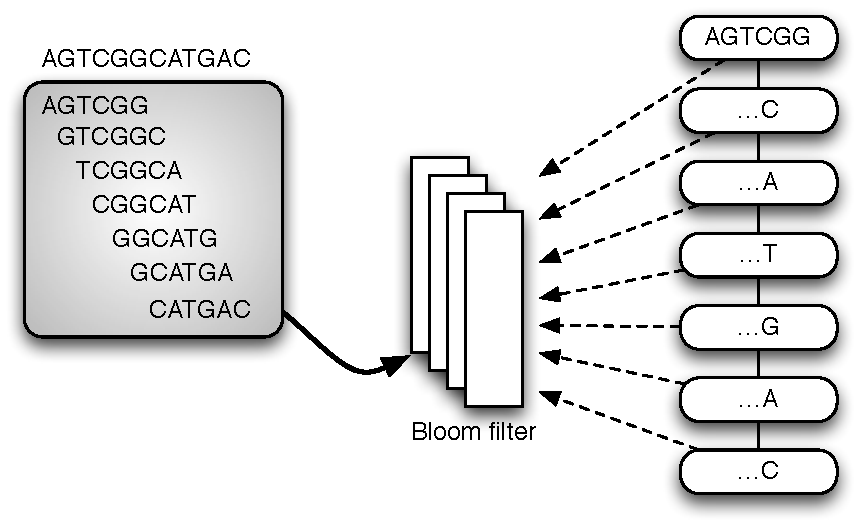
\includegraphics[width=5in]{bloomgraph}
\caption{Storing de Bruijn graphs in Bloom filters.  Longer sequences are broken down into k-mers (here, k=6) and stored in the Bloom filter.
The graph is traversed by starting with a k-mer and then testing all possible 1-base pre- and post-fixes for presence in the Bloom filter.}

\label{fig:bloomgraph}
\end{figure}

\begin{figure}
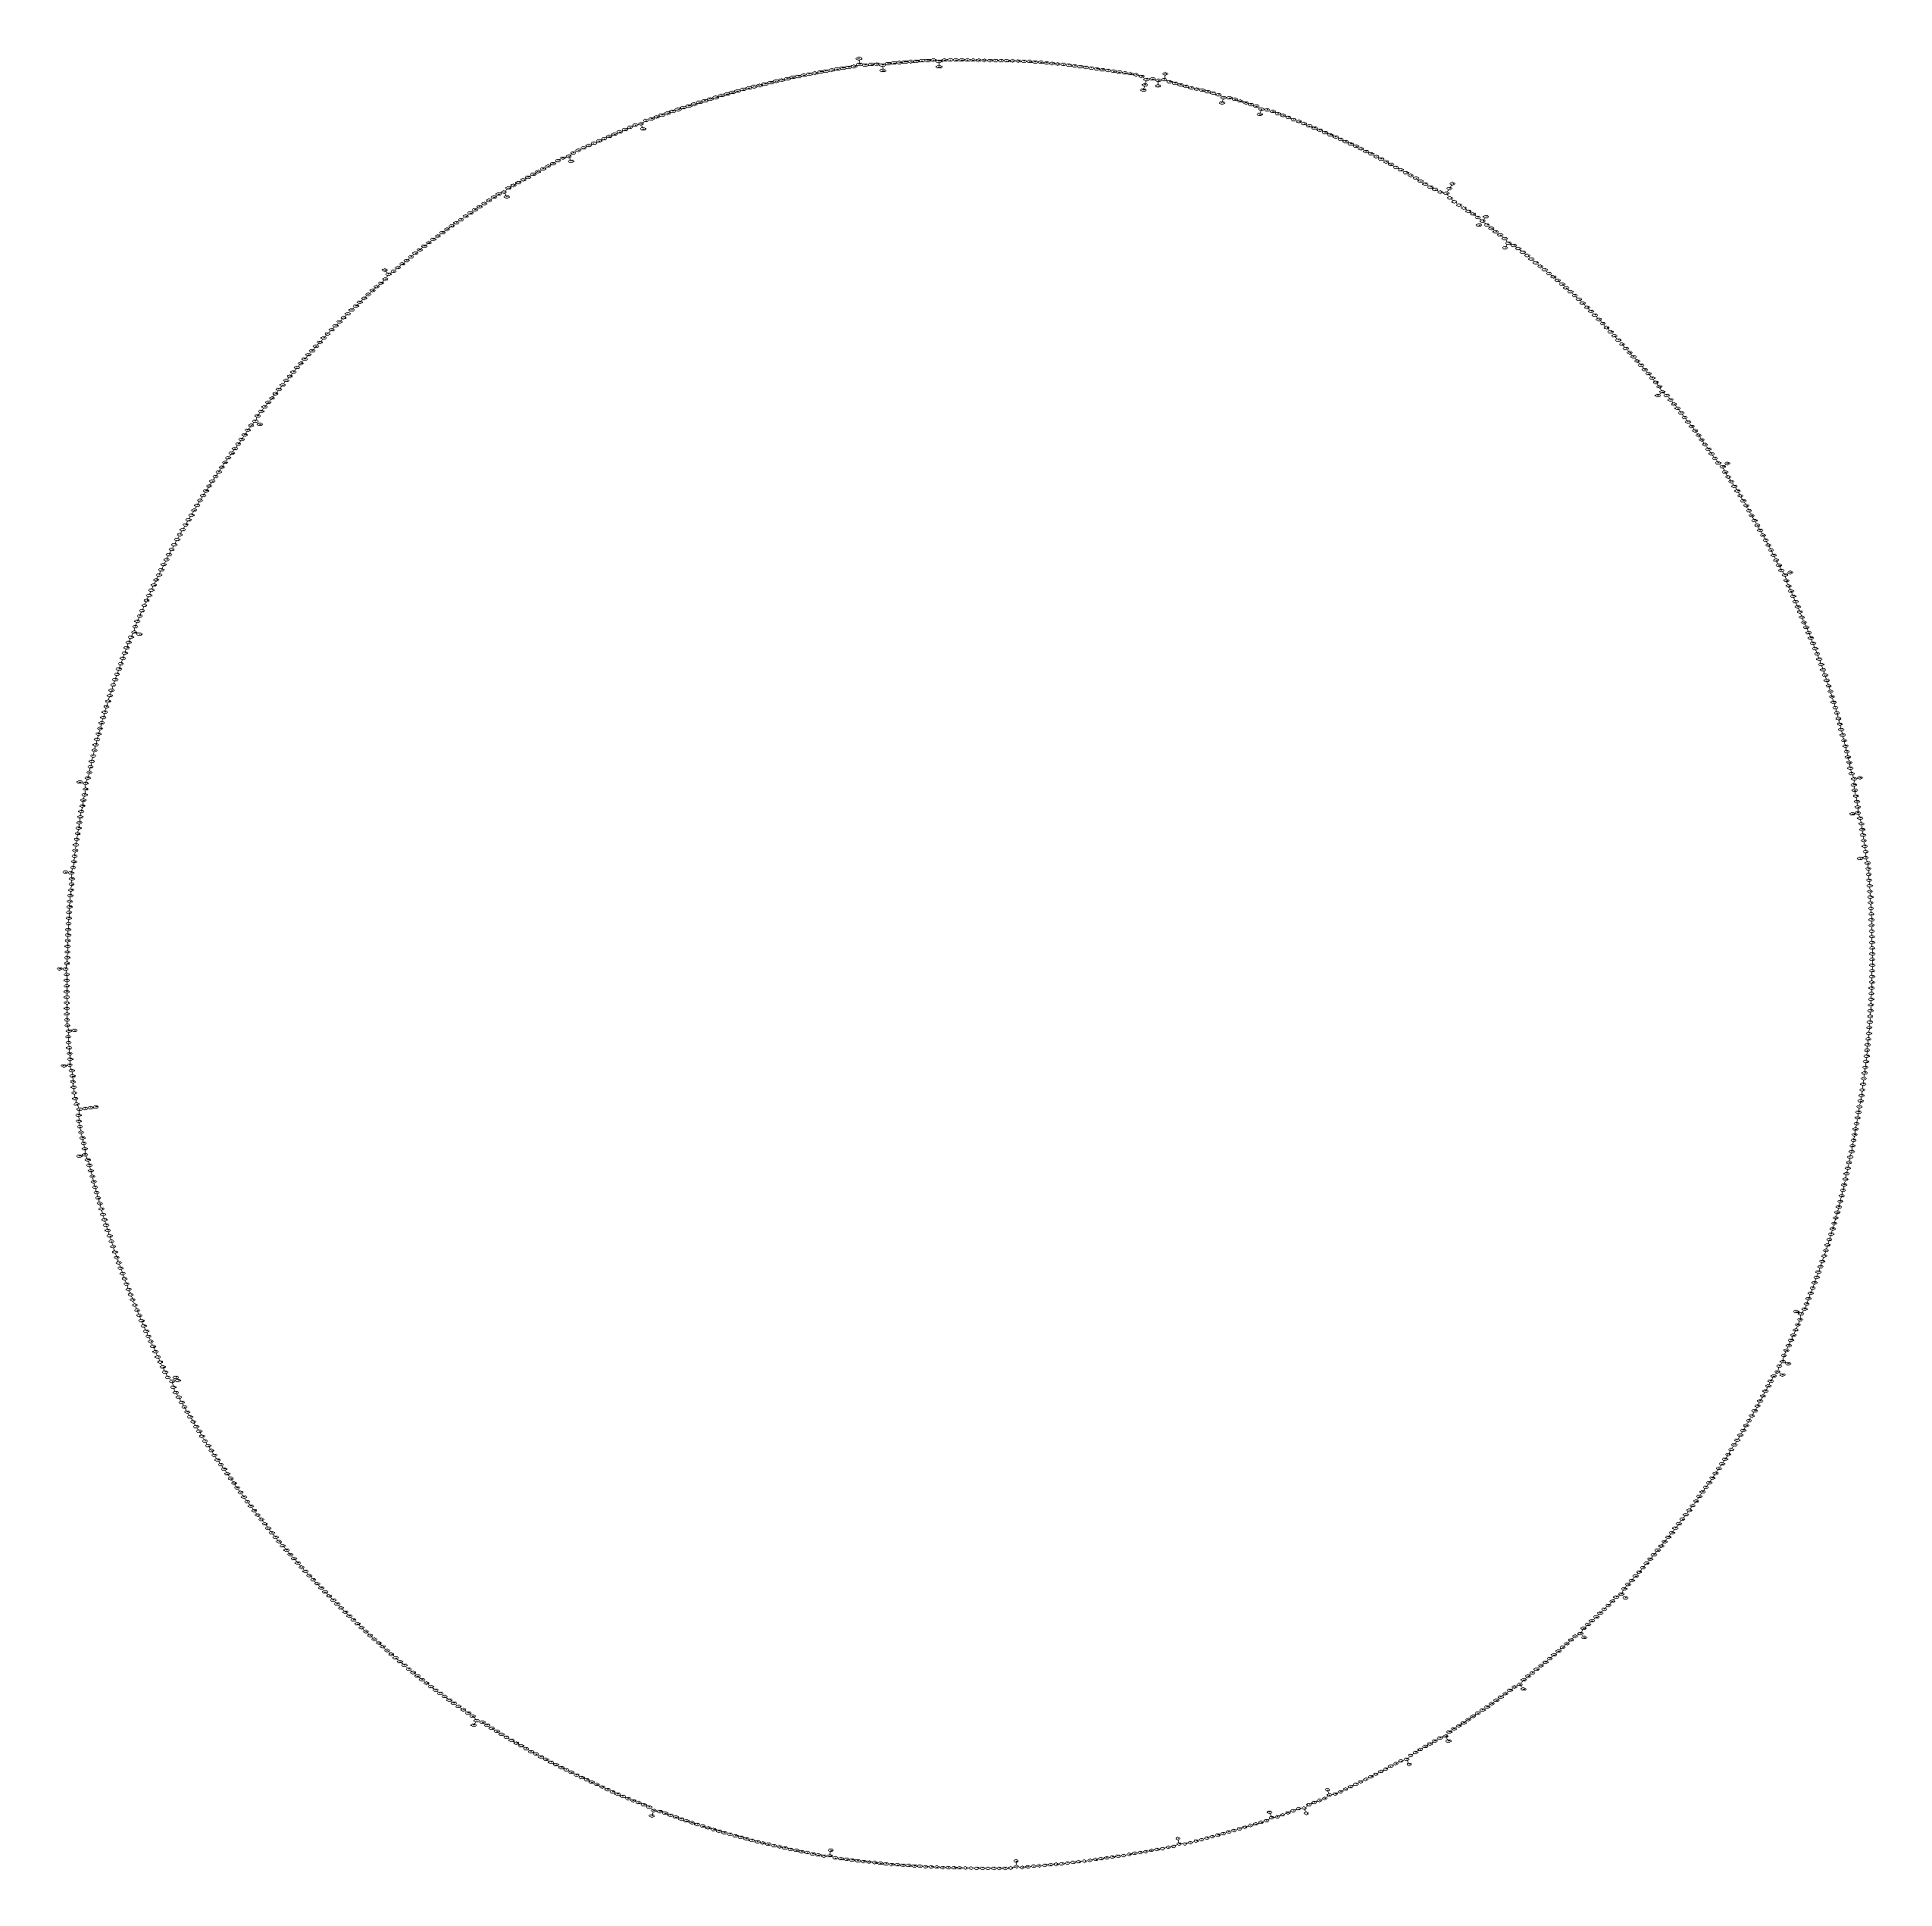
\includegraphics[width=2in]{figures/f3b001}
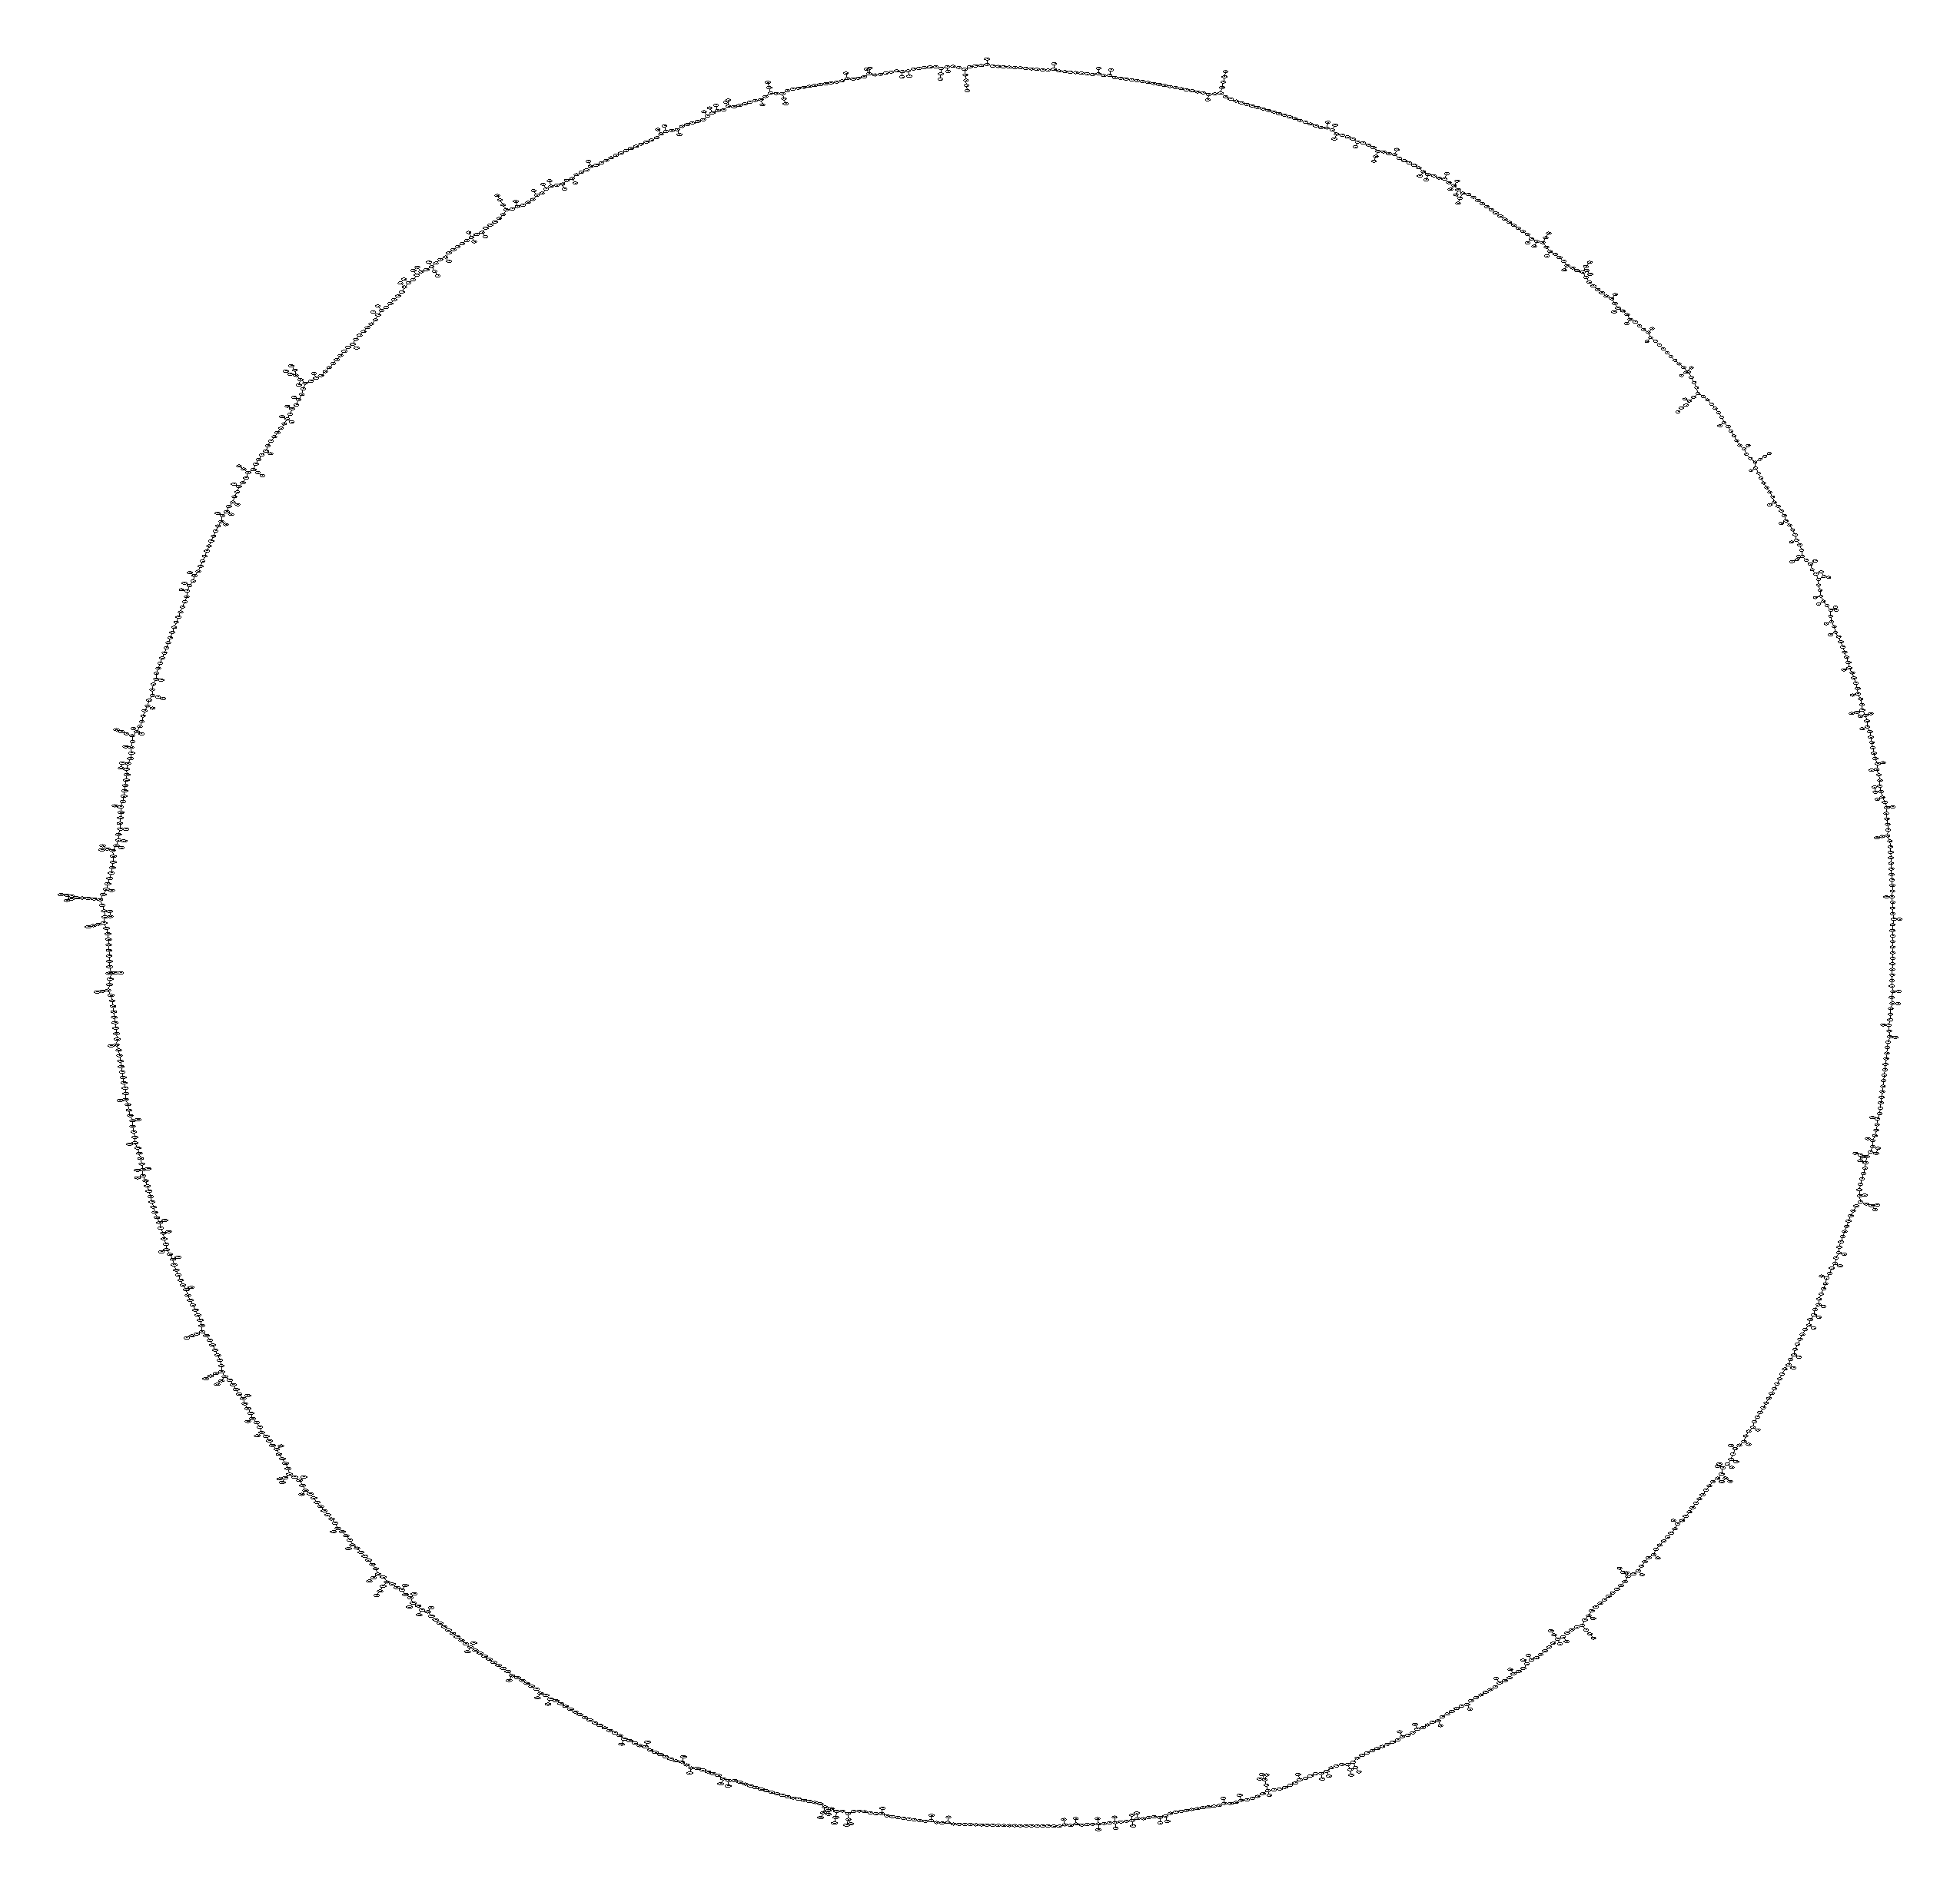
\includegraphics[width=2in]{figures/f3b005}
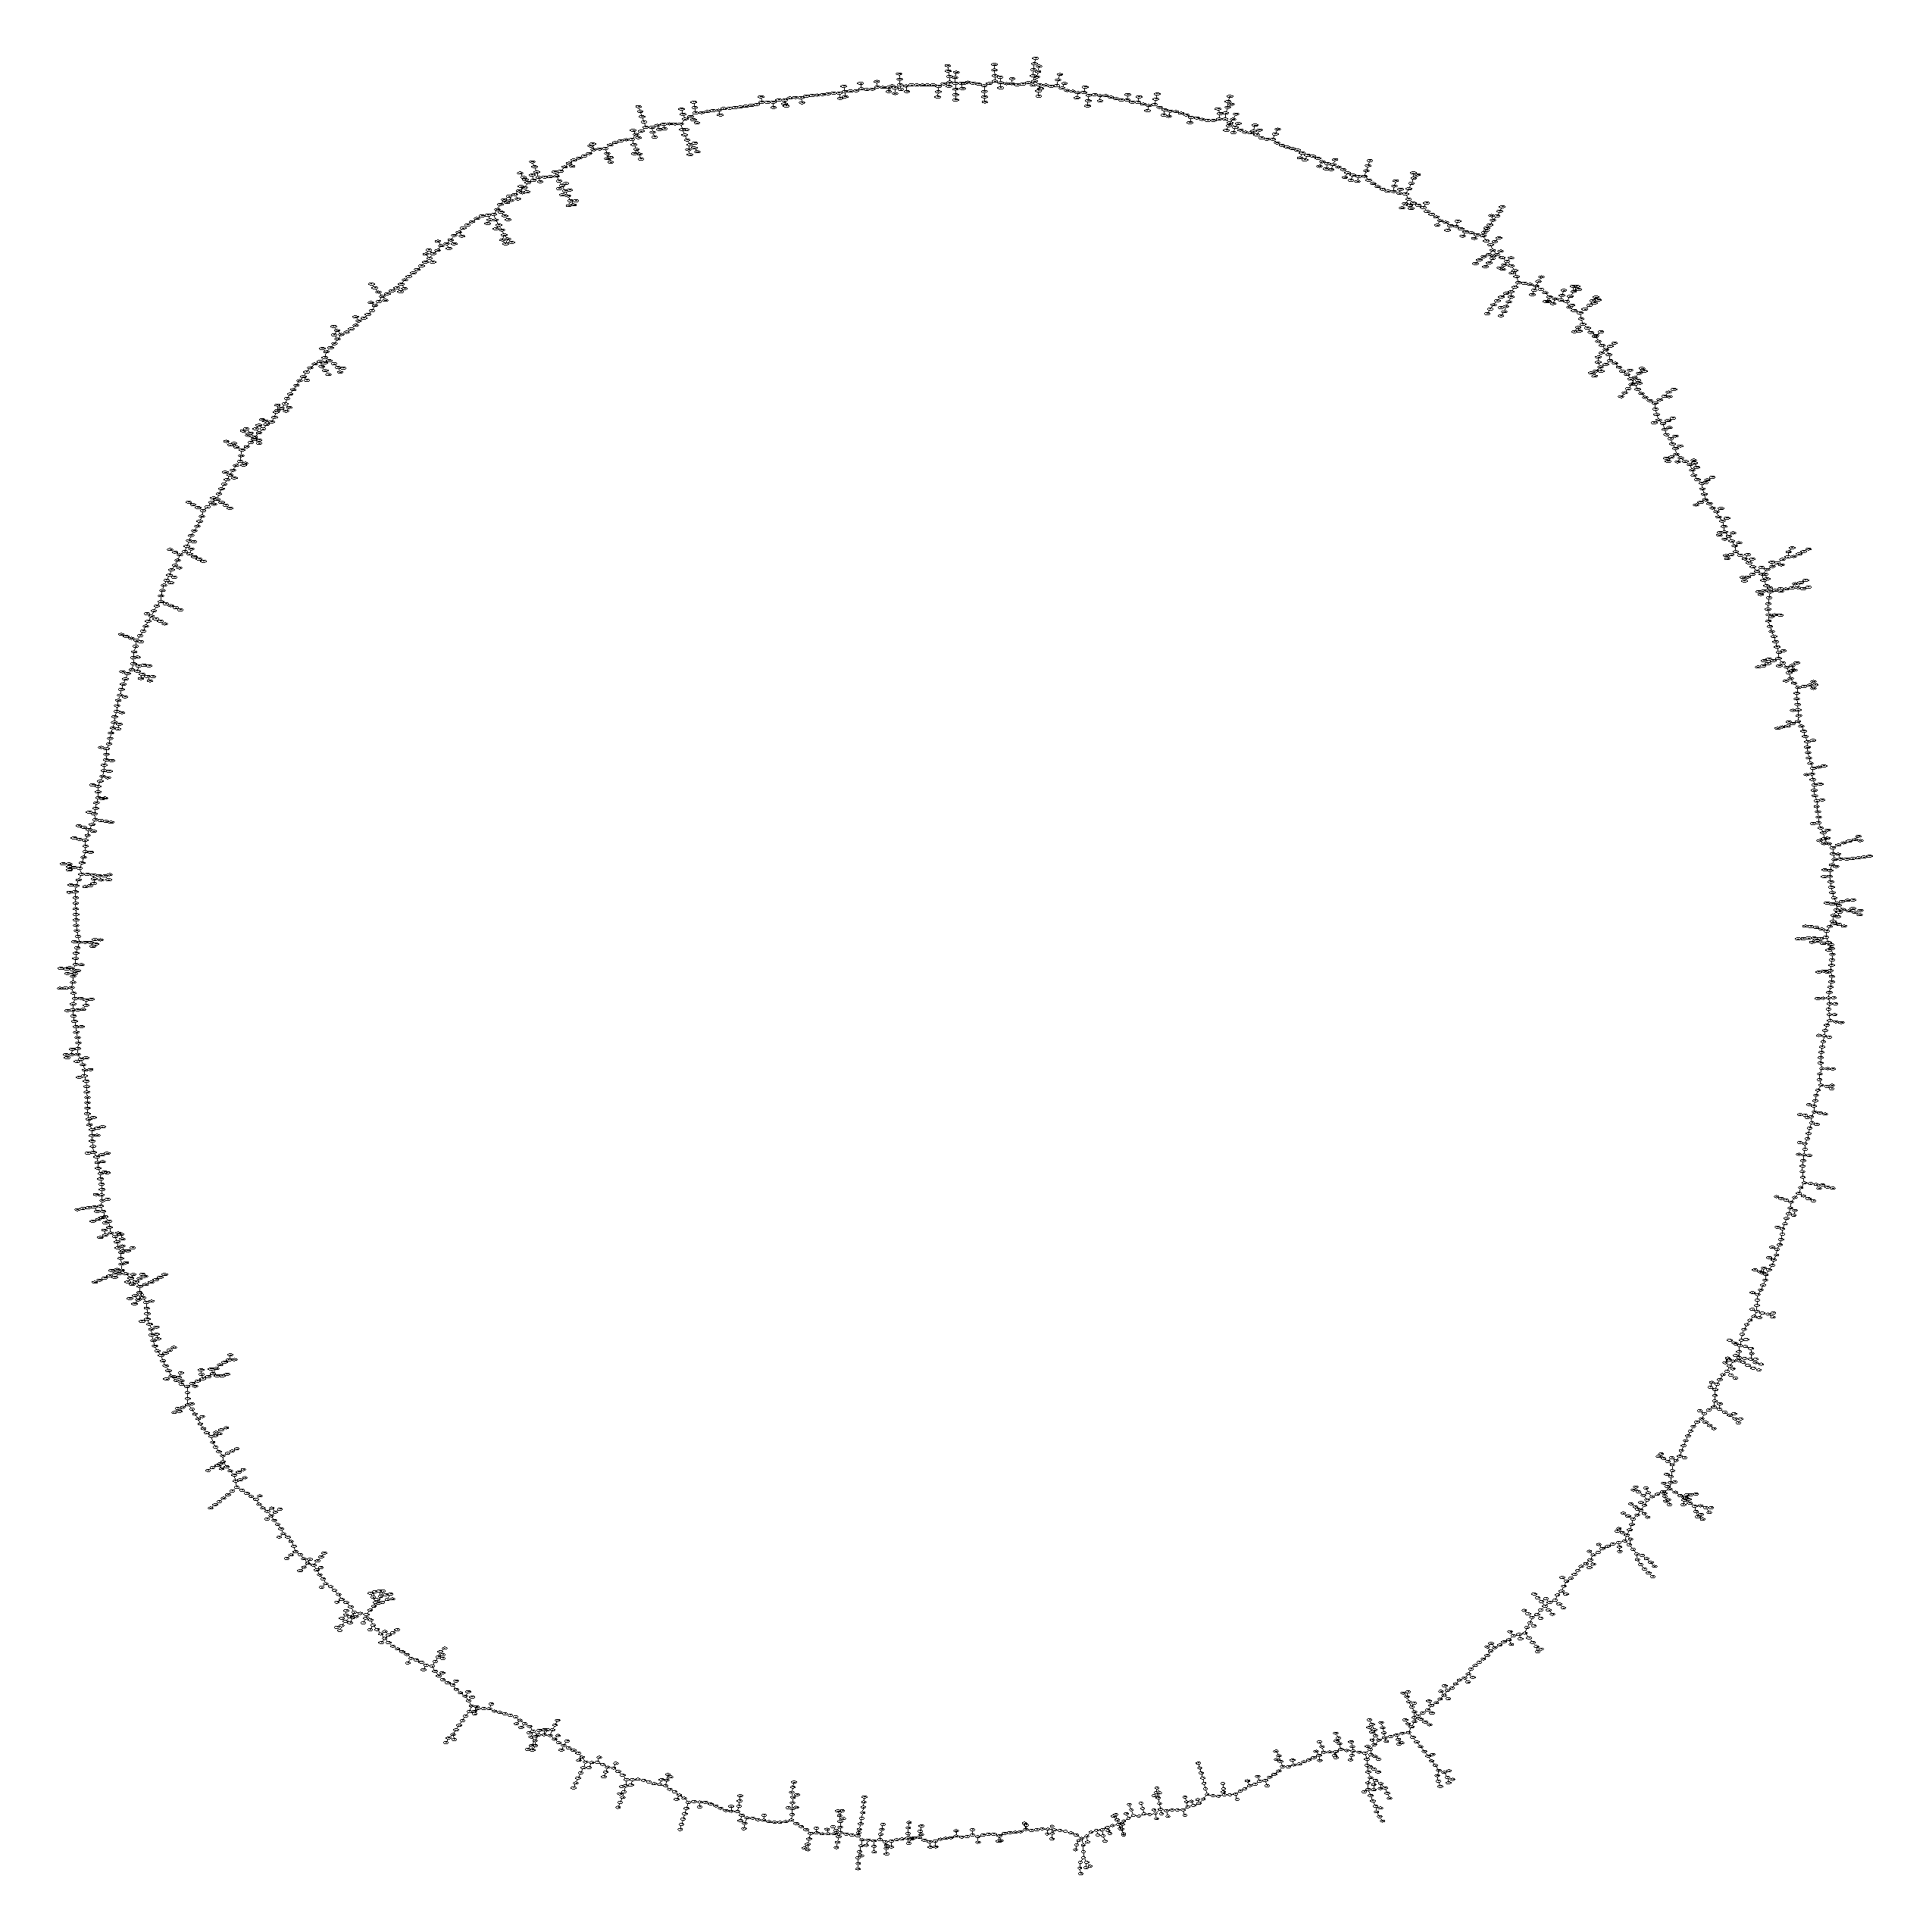
\includegraphics[width=2in]{figures/f3b010}
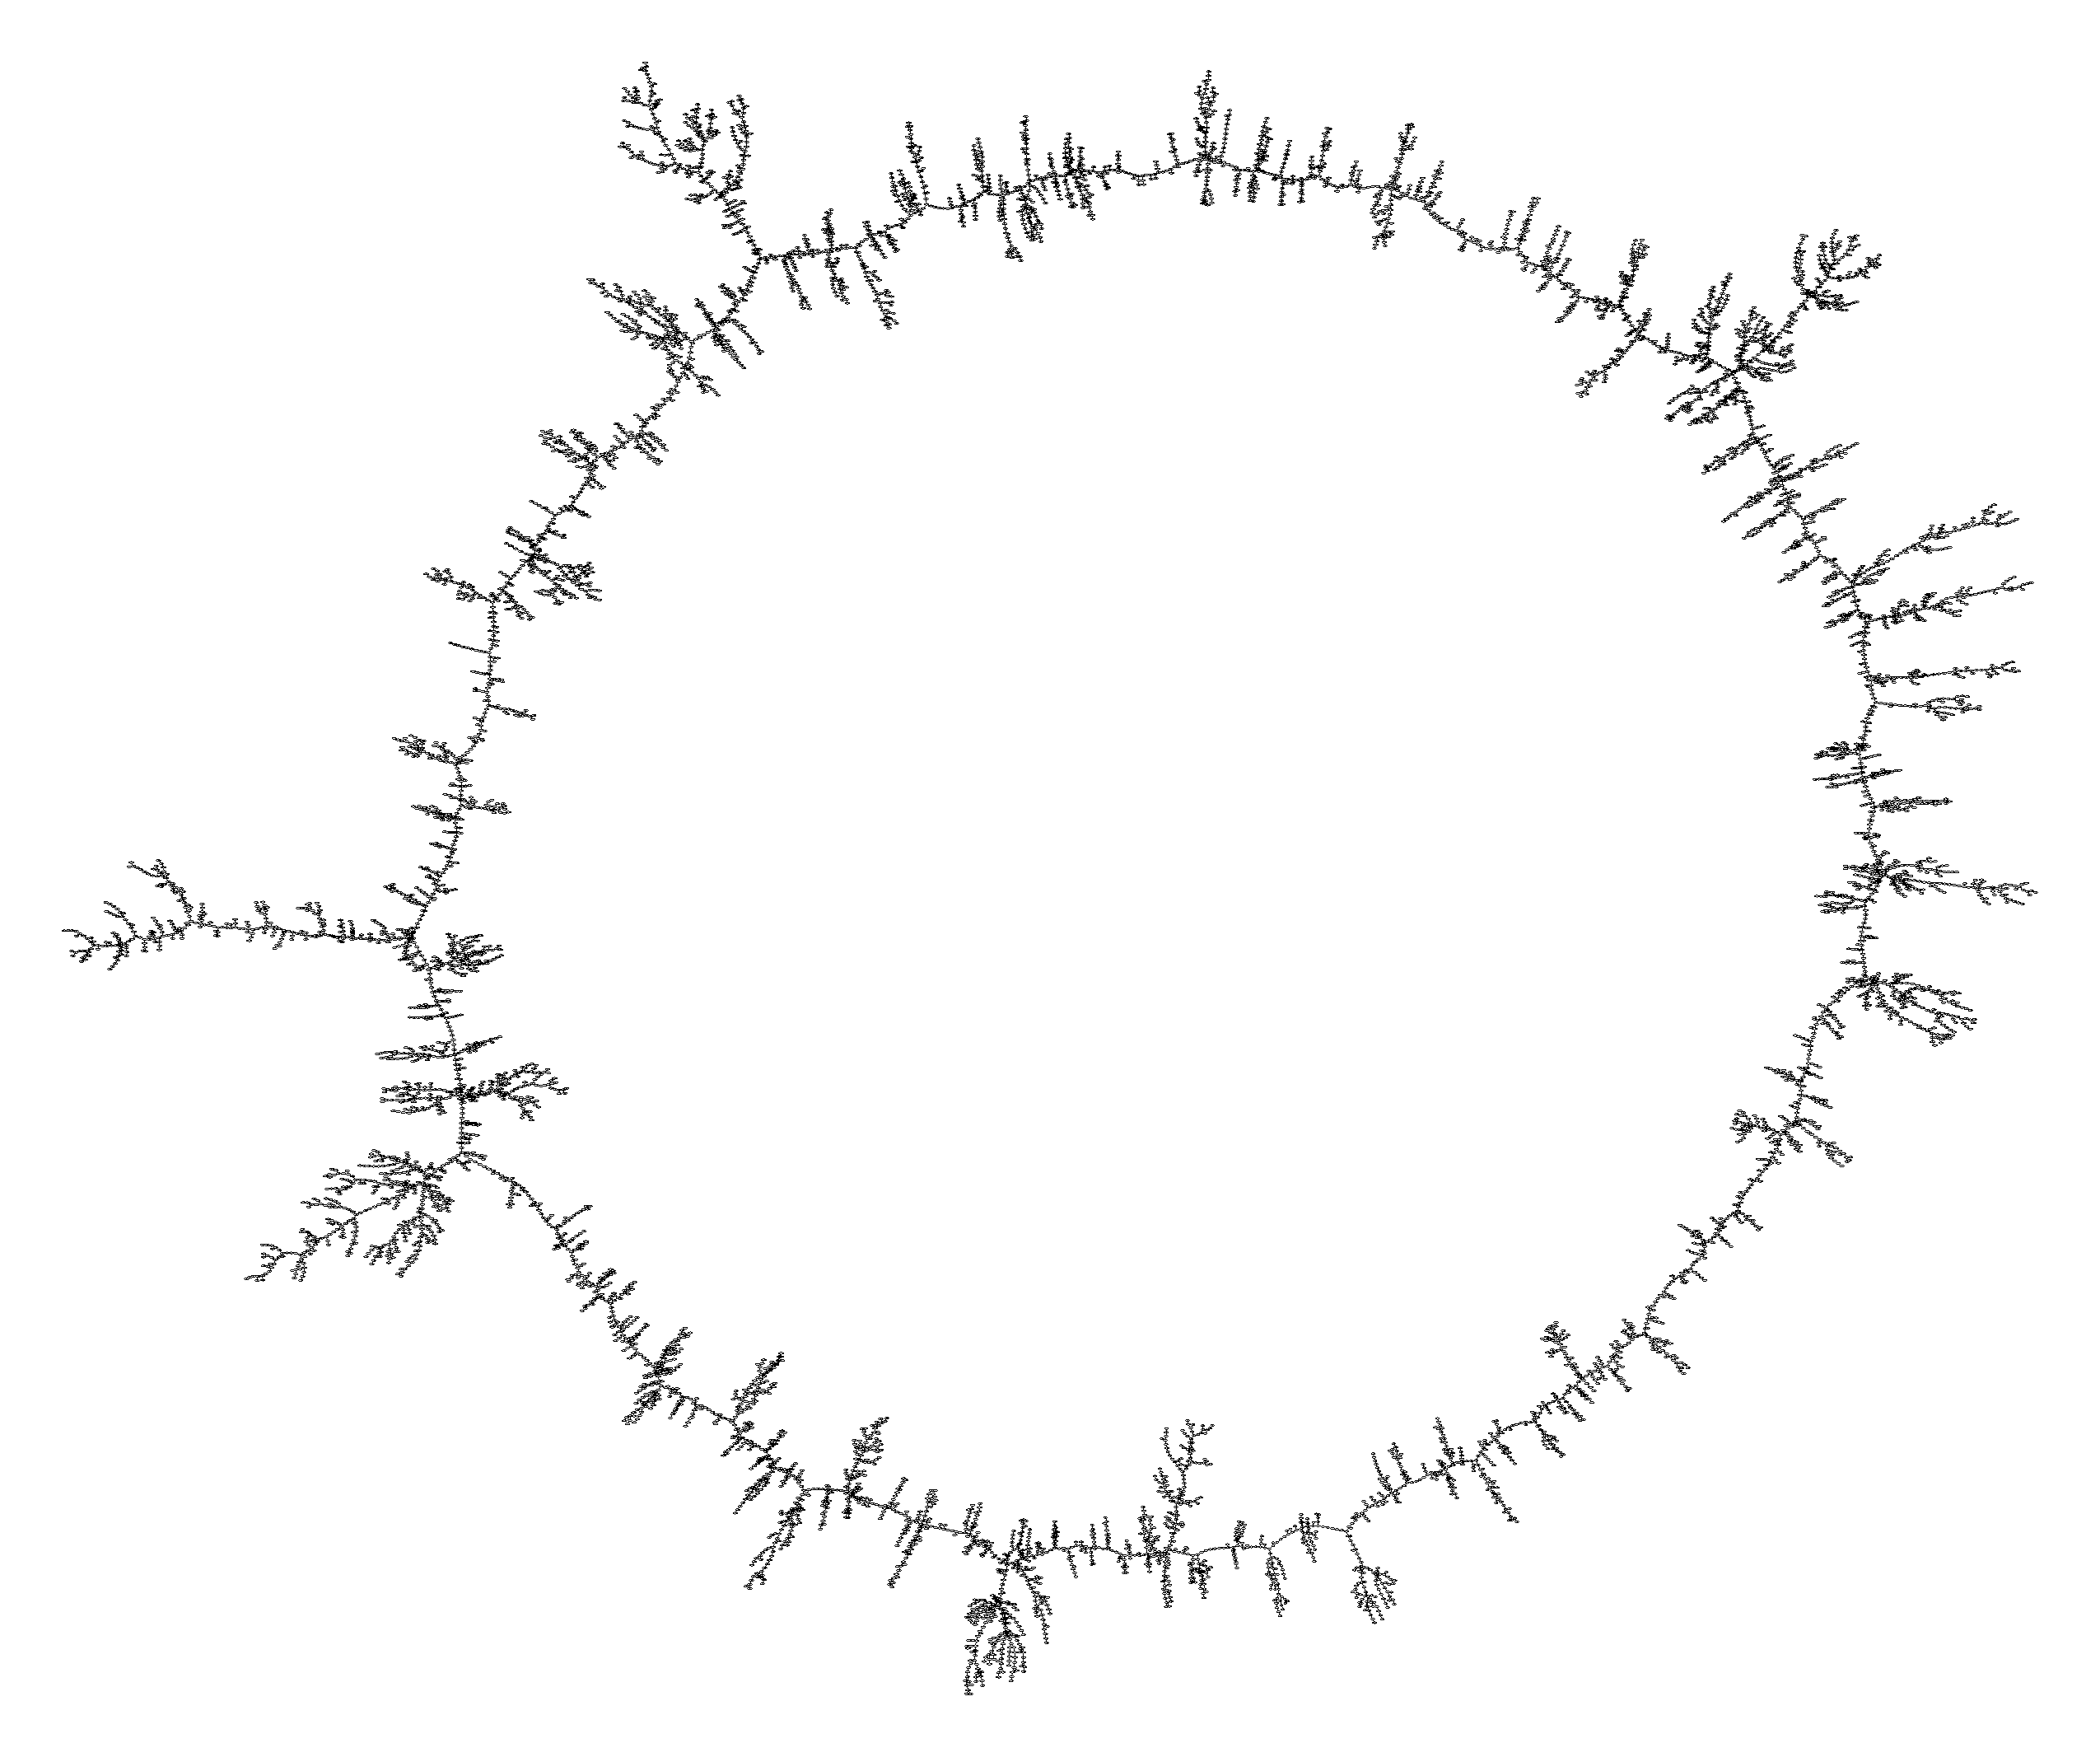
\includegraphics[width=2in]{figures/f3b015}
\caption{Graph visualizations demonstrating the decreasing 
fidelity of graph structure with increasing false positive rate. From 
top left to bottom right, the false positive rates are 0.01, 0.05, 0.10, 
and 0.15.}
\label{fig:circles}
\end{figure}

\begin{figure}
\center{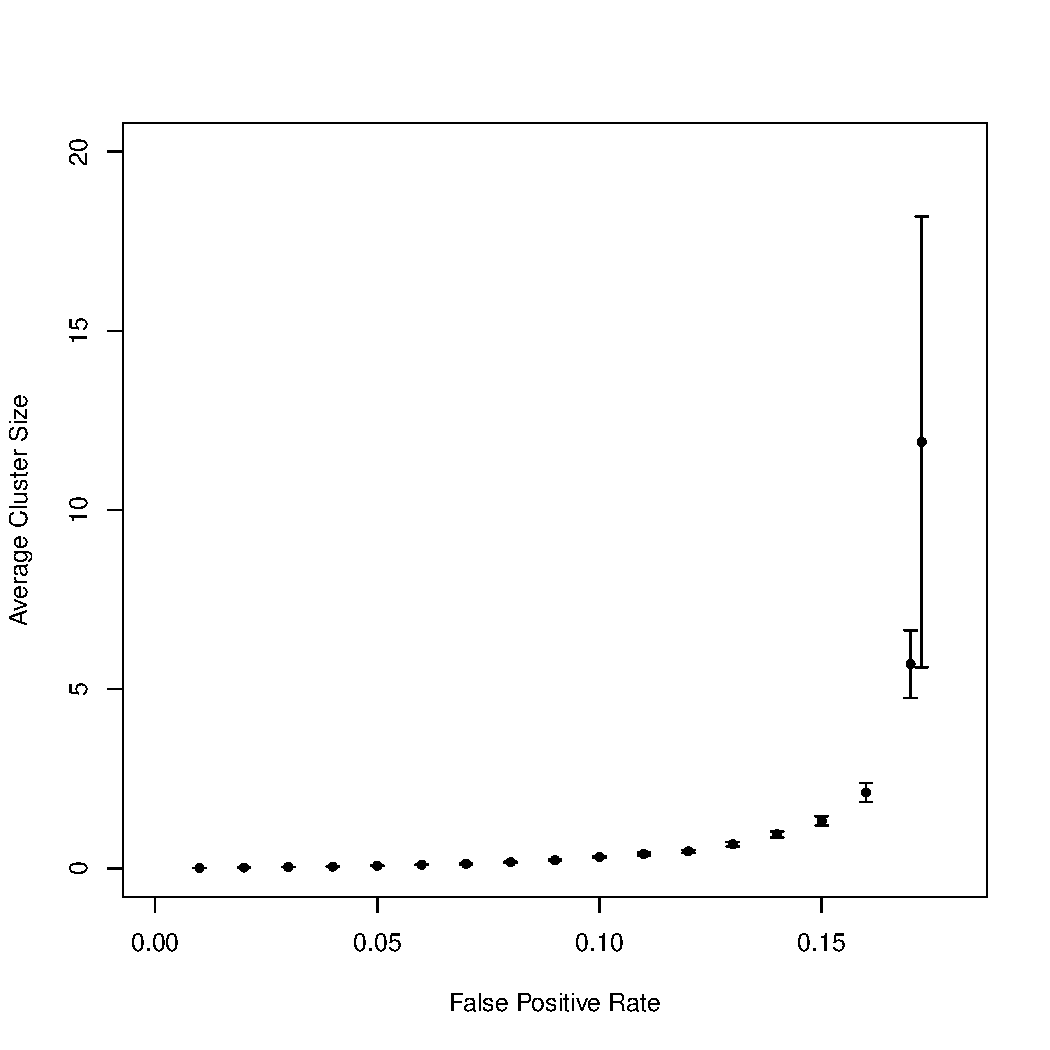
\includegraphics[width=5in]{newclust}}
\caption{Average cluster size versus false positive rate. The average 
cluster size sharply increases as the false positive 
rate approaches the percolation threshold.
}
\label{fig:clustersize}
\end{figure}

\begin{figure}
\center{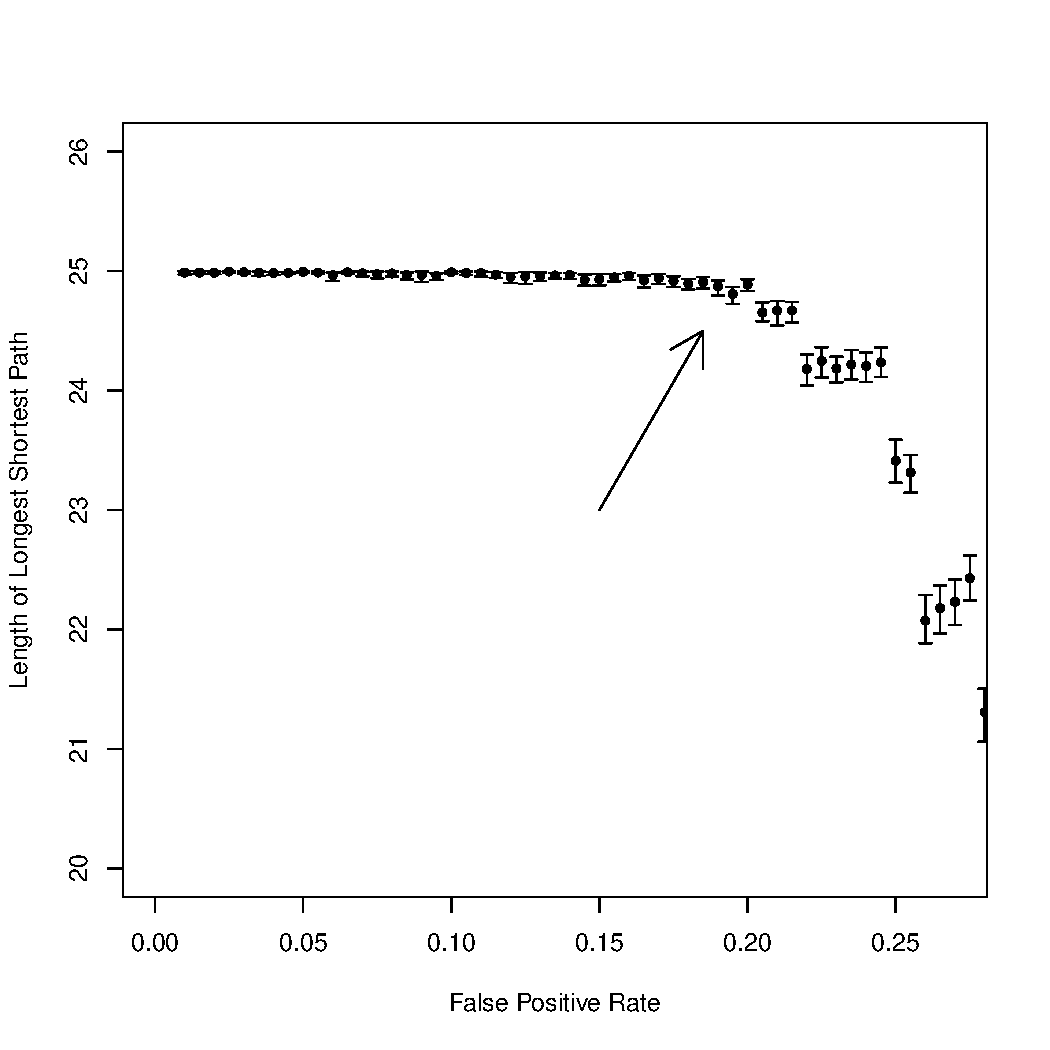
\includegraphics[width=5in]{figures/newdiam}}

\caption{Length of Longest Shortest Path by False Positive Rate. The
  length of the longest shortest path of randomly generated 58bp long
  circular chromosomes in 8-mer space for different false positive
  rates. Only real (non-error) k-mers are considered for starting and
  ending points.}
\label{fig:diam}
\end{figure}

\begin{figure}
\center{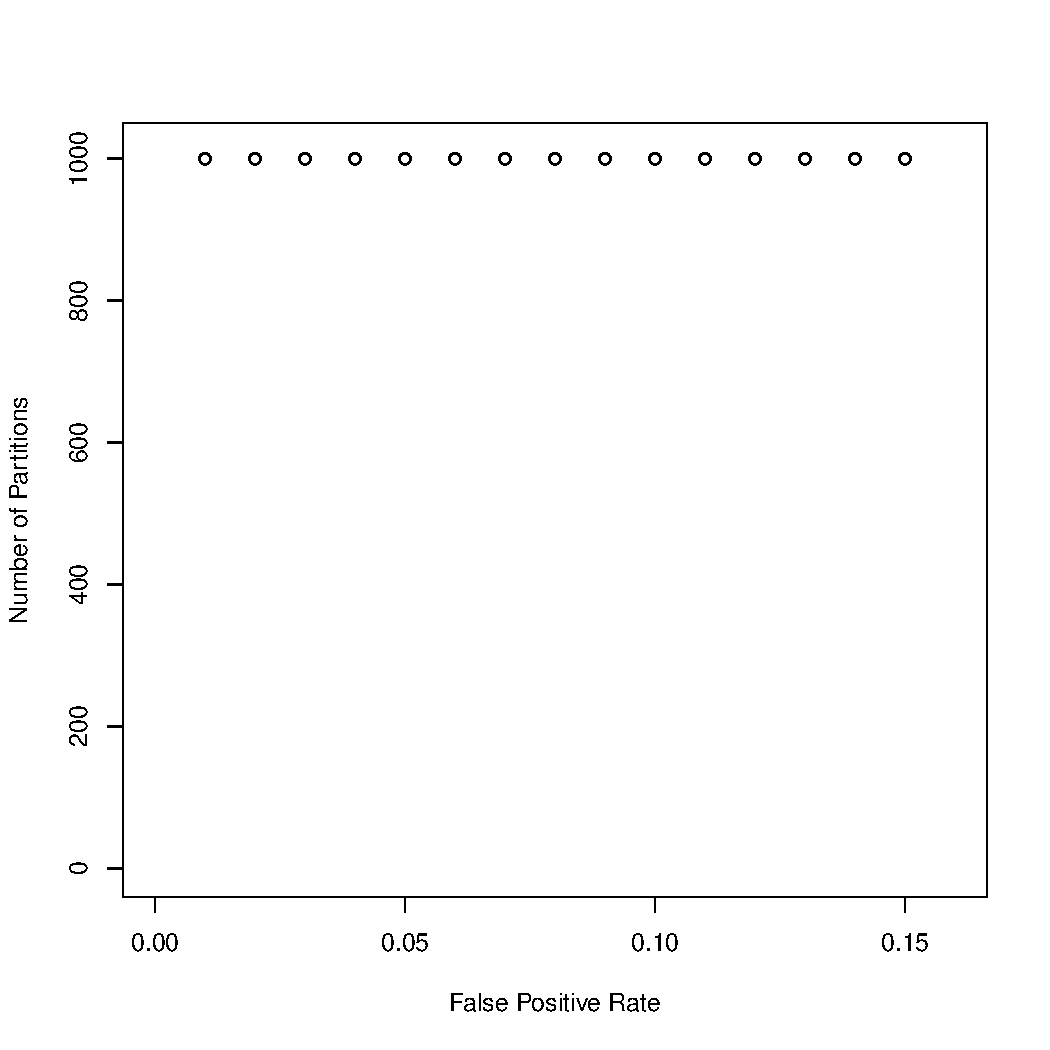
\includegraphics[width=5in]{figures/newpart}}

\caption{Number of Partitions by False Positive Rate. The graph shows
  the resulting number of partitions for a simulated dataset with
  1,000 contigs of 10,000 bp each (circles). For $n=5$ different
  combinations of hash table sizes, there was no variation in results
  for the simulated dataset.}

\label{fig:partfp}
\end{figure}

% Memory
%  use is maximum memory required in gigabytes during partitioning,
%  with the given improvement ratio over using the ABySS assembler on
%  the unpartitioned data, which required 33 GB.  N partitions is the
%  total number of partitions containing more than 500 k-mers, and D is
%  the largest partition size in reads.}

\begin{table*}
\centering
\caption{Bits per k-mer for various false positive rates.}
\begin{tabular*}{\hsize}{@{\extracolsep{\fill}}cccc}
\hline
False positive rate & Bits/k-mer \\ \hline
0.1 \% & 14.35 \cr
1 \% & 9.54 \cr
5 \% & 6.22 \cr
10 \% & 4.78 \cr
15 \% & 3.94 \cr
20 \% & 3.34 \cr
\hline\end{tabular*}
\label{table:bitskmer}
\end{table*}

\begin{table}
\centering

\caption{Effects of loading \emph{E. coli} data at different false positive rates}
\begin{tabular*}{\hsize}{@{\extracolsep{\fill}}ccccccc}
\hline
Graph & Total k-mers & False k-mers & Deg $\ge 2$ & \% Real & Mem (bits) \\ \hline
\emph{E. coli} at 0\% & 4,530,123 & 0 & 50,605 & 100 & $1.71 \times 10^{10}$ \\
\emph{E. coli} at 1\% & 4,814,050 & 283,927 & 313,844 & 94.1 & $4.34 \times 10^7$ \\
\emph{E. coli} at 5\% & 6,349,301 & 1,819,178 & 1,339,102 & 71.3 & $2.82 \times 10^7$ \\
\emph{E. coli} at 15\% & 31,109,523 & 26,579,400 & 10,522,482 & 14.6 & $1.79 \times 10^7$ \\
Reads at 0\% & 45,566,033 & 41,036,029 & 7,700,483 & 9.9 & $1.71 \times 10^{10}$ \\
Reads at 1\% & 48,237,038 & 43,707,032 & 9,771,028 & 9.4 & $4.37 \times 10^8$ \\
Reads at 5\% & 62,094,757 & 57,564,749 & 18,116,934 & 7.3 & $2.84 \times 10^8$ \\
Reads at 15\% & 235,654,877 & 231,124,854 & 85,813,621 & 1.9 & $1.8 \times 10^8$ \\
\hline
\end{tabular*}
\label{table:ecoli}
\end{table}

\begin{table*}
\centering
\caption{Partitioning results on a soil metagenome at k=31.}

\begin{tabular*}{\hsize}{@{\extracolsep{\fill}}cccc}
False positive rate & Total memory use (improvement) & Largest partition size in reads \cr
\hline
1\% & 2.0gb (16.5x) & 344,426 \cr
5\% & 1.55gb (21.3x) & 344,426 \cr
10\% & 1.43gb (23.1x) & 344,428 \cr
15\% & 2.2gb (15x) & 344,784 \cr
\hline
\end{tabular*}

\label{table:parts}
\end{table*}

%% @@effects of local graph elaboration on partitioning/traversal alg?
%% @@graphsize filtering vs partitioning?
%% @@change mem/bits to mem/bytes.
%% @@go back and refer to tables and figures in discussion, too.

\end{document}
